\documentclass{article}

\usepackage{mathtools,amsfonts}
\usepackage{enumitem}
\usepackage{fullpage}
\usepackage{fancyvrb}
\usepackage{hyperref}


\begin{document}
\thispagestyle{empty}

\begin{center}
  \textbf{\Large <LEVEL> Test <NUMBER>}
  % LEVEL is Senior, Intermediate or Beginner
  % NUMBER is the test number: 1, 2, etc.
  \\ \vspace{1em}
  \textbf{\large Stellenbosch Camp 2022}
  \\ \vspace{1em}
  \textbf{\large Time: $2\frac{1}{2}$ hours}
\end{center}

\bigskip

\begin{enumerate}[itemsep=\fill]

\item % Source of problem
Problem statement


\item %
For nonzero real numbers $a$, $b$, and $c$, show that
\[ \frac{a}{b} +\frac{b}{c} +\frac{c}{a} = \frac{a}{c} +\frac{c}{b} +\frac{b}{a} \]
if and only if two of $a$, $b$, and $c$ are equal.

\textbf{Solution:} Observe the following computation:
\begin{align*}
\frac{a^{2}b + b^{2}c + c^{2}a}{abc} & = \frac{a^{2}c + b^{2}a + c^{2}b}{abc}\\
 0 & = \frac{a^{2}c + b^{2}a + c^{2}b -(a^{2}b + b^{2}c + c^{2}a)}{abc} \\
 0 & = \frac{abc + a^{2}c + b^{2}a + c^{2}b - (a^{2}b + b^{2}c + c^{2}a+abc)}{abc} \\
 0 & = \frac{(a-b)(b-c)(c-a)}{abc} \\
\end{align*}
One of $a-b$, $b-c$, $c-a$ must be zero, showing that some pair among $a$, $b$, $c$ must be equal.

\item % Tsimerman
Can you tile a $10\times 10\times 10$ cube with $4\times 1\times 1$ blocks? (Standard tiling rules apply---cover the whole volume, no overlaps, etc.)

\textbf{Solution:} The answer is no. Consider the following colouring: there are 10 `layers' to the cube. Label these layers from 1 to 10. For layers 1,2,5,6,9,10, we colour the layer as follows:
\begin{center}
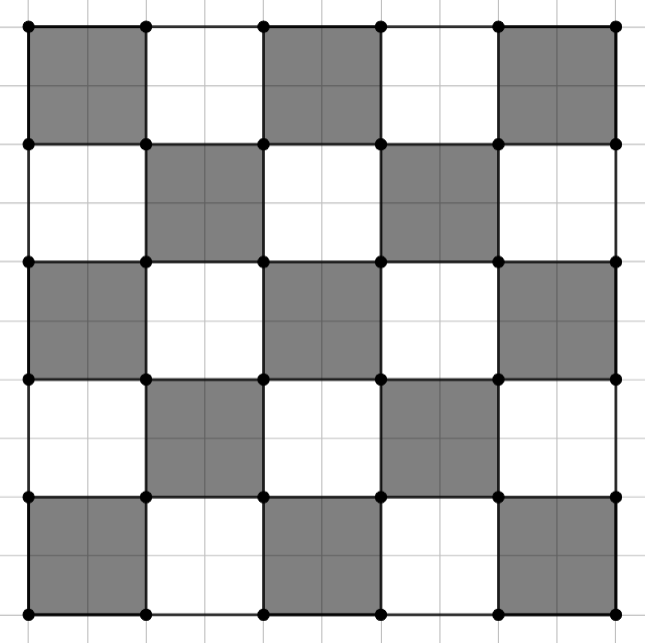
\includegraphics[scale=0.5]{Capture.png}
\end{center}
For layers 3,4,7,8, we invert these colours.\\
We note that each $4\times 1\times 1$ covers exactly 2 shaded blocks and 2 unshaded.\\
But counting the total number of shaded blocks gives 504, while there are 496 unshaded blocks.\\
Thus, we can not tile the shape as requested. 


\item % 


\item % 

\end{enumerate}


% ASCII art
\centering
\small
\begin{BVerbatim}
% Insert art here
\end{BVerbatim}

\end{document}
